%& -shell-escape
%\documentclass[a4paper]{aa}
\documentclass[printer]{aa}
% \documentclass{article}
\usepackage[pagebackref,colorlinks,citecolor=blue,urlcolor=blue,linkcolor=blue]{hyperref}
\usepackage[varg]{txfonts}
\usepackage{graphicx}
\usepackage{natbib}
\usepackage{amssymb}
\usepackage{amsmath}
\usepackage{tikz}
\usetikzlibrary{arrows,positioning,shapes} %,optics}

%\usepackage[squaren,Gray]{SIunits}
\usepackage{siunitx}
%\usepackage{units} % nicefrac
%\newcommand{\units}[1]{$\mathrm{#1}$}

\newcommand{\Oldthorlabs}{SM05PD1B}
\newcommand{\Newthorlabs}{SM05PD3A}

\newcommand{\todo}[1]{\textbf{\textcolor{red}{[#1]}}\xspace}

\usepackage[outputdir={fig},debug]{dot2texi}
\usepackage{draftwatermark}
\usepackage{xspace}
\SetWatermarkText{DRAFT}
\SetWatermarkScale{6}
\SetWatermarkLightness{0.9}
\newcommand{\angexp}{\circ{a}}
\newcommand{\texp}{\ensuremath{\tau}\xspace}
\newcommand{\FixMe}[1]{\textbf{\textcolor{red}{[#1]}}\xspace}
\newcommand{\SZF}[1]{\textbf{\textcolor{blue}{[#1]}}\xspace}
\newcommand{\MARC}[1]{\textbf{\textcolor{green}{[#1]}}\xspace}
\graphicspath{{fig/}}
\makeatletter
\newcommand*\ExpandableInput[1]{\@@input#1 }
\makeatother
\DeclareMathOperator*{\med}{med}
\title{The StarDICE absolute flux calibration experiment: Characterisation of the photometric instrument with a collimated beam projector}

\author{Collaboration Boston Paris}

\abstract{}{}{}{}

\begin{document}

\maketitle

%\section{Currently happening}
%
%\begin{itemize}
%\item SC linearity
%\item pinhole choice
%\item dark current caracterization
%\item Photo-diode change
%\end{itemize}

\tableofcontents

\section{Introduction}


\section{Laboratory setup}

\subsection{StarDice}

\todo{Marc} The StarDICE photometric instrument (SPI) consists in a
Newton telescope with a primary mirror of $40$cm diameter (16'') and
$1.6$m focal length ($f/D = 4$). The focal plane hosts an Andor Ikon-M
954 camera, equipped with a thermoelectrically cooled, deep depleted
and back illuminated CCD sensor (E2V DU934P). The active area of the
sensors is $13.3\times13.3 mm$ divided in $1024\times 1024$ square
pixel of $13\mu m$ side. In this baseline setup, the pixel resolution
is $1.68$ arcsec and the field of view $28.6\times28.6$ arcmin.

The 11cm diagonal is oversized to ensure the fully-illuminated plane
extends over the sensor with a confortable margin in all optical
configurations.

[-0.9240625, -13.120000000000001]

\begin{itemize}
\item Filter-CCD distance: max 40.80 mm, min 26.80 mm
\item field of view $30'x30'$
\item Custom built mount
\item filters $ugrizy$
\end{itemize}



\begin{figure*}[!h]
\centering
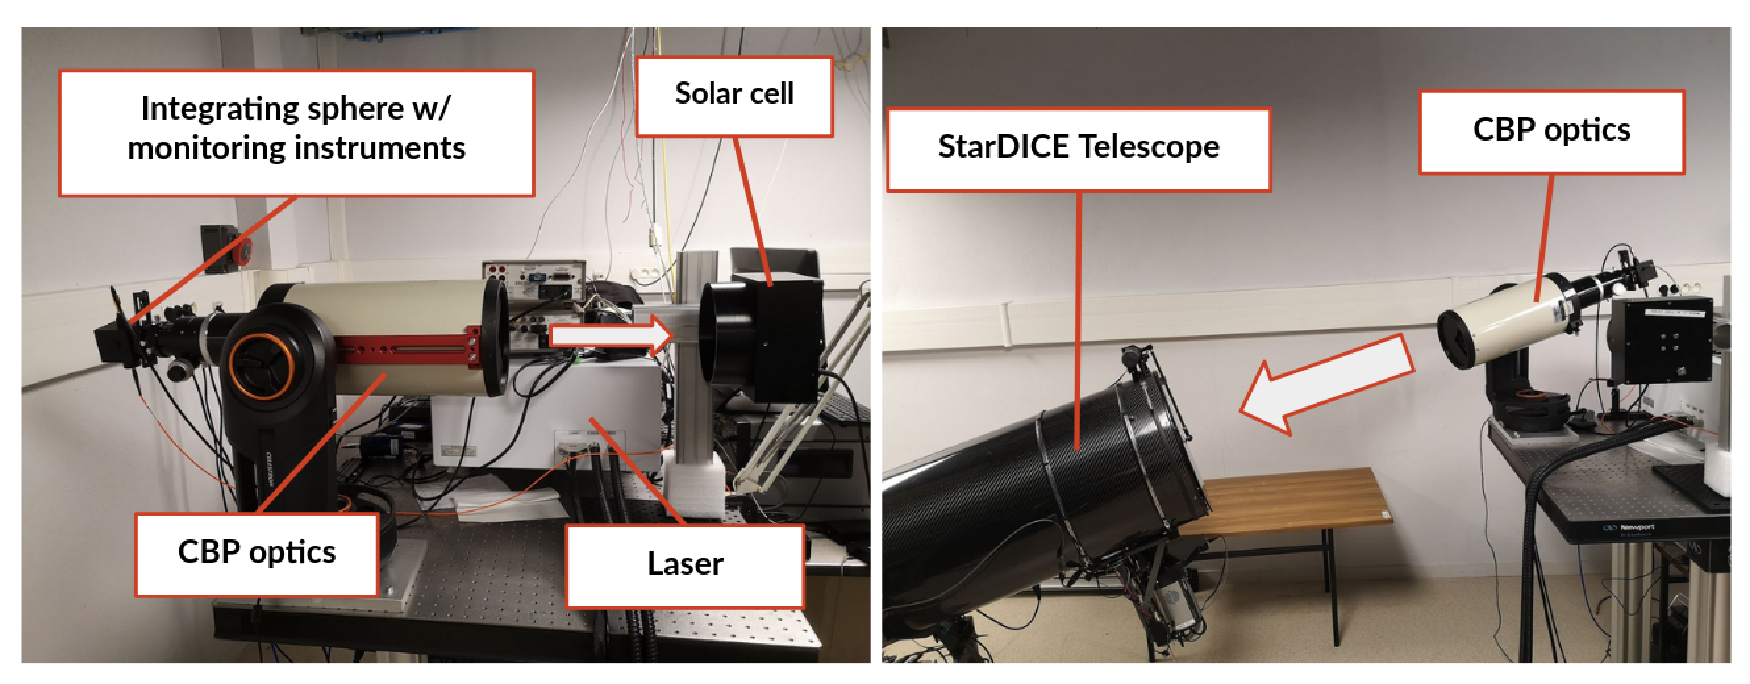
\includegraphics[width=\textwidth]{cbp_setup}
\caption{General setup of the CBP. Left: the CBP telescope pointing at the solar cell, with its quart disk aperture frame. Middle: the light injection system. Right: the CBP telescope pointing toward the \SD telescope.}\label{fig:cbp_setup}
\end{figure*}

\subsection{CBP setup}


\todo{Jeremy}

The Collimated Beam Projector is basically an artificial monochromatic star. The light source is an Ekspla NT252 tunable laser, using a pump laser at \SI{532}{\nano\meter} and non-linear crystals to produce powerful monochromatic pulses from 335 to \SI{2600}{\nano\meter}. The pulse duration is fixed and lies between 1 to \SI{4}{\nano\second} with an energy of \SI{1.1}{\milli\joule} in the near infra-red. The pulses are shot in bursts, with a fixed frequency of \SI{1}{\kilo\hertz} and a maximum linewidth below \SI{10}{\per\cm}. This converts into a maximum spectroscopic width below \SI{0.4}{\nano\meter} around \SI{600}{\nano\meter}. This is an upper limit quoted by the manufacturer, but measurements taken using a similar laser show bandwidths going from \SI{0.08}{\nm} to \SI{0.48}{\nm} in the 350 to \SI{1100}{\nm} range \citep{woodward2018}. The standard deviation of pulse energy is around 2.5\%. This laser is composed of three stages to operate (from 335 to \SI{669}{\nano\meter}, from 670 to \SI{1064}{\nano\meter} and above \SI{1064}{\nano\meter}), which results in three different regimes of power and light contamination in the CBP. This laser was chosen for the offered wide wavelength range and the high pulse energy, which is important for the CBP calibration with the solar cell. 

The laser output is focused into an optical fibre injection system. Before, a filter wheel containing three different broad bandpass filters helps purifying the laser light from pump photons or other resonances in the system. In particular, we use a pass-blue filter BrightLine Multiphoton FF01-680/SP-25 in the regime 530 to \SI{645}{\nano\meter} to remove \todo{a bien justifier}, a pass-red filter RazorEdge LP03-532RU-25 to filter the \SI{532}{\nano\meter} pump photons in the regime 645 to \SI{1074}{\nano\meter}, and a pass-infrared filter RazorEdge LP02-1064RU-25 above \SI{1074}{\nano\meter} to filter \SI{1064}{\nano\meter} photons appearing in this regime. All this optical stage is packed inside a black metallic box to prevent room light contamination.


The high UV transmission optical fibre arrives into a \SI{50}{\mm} diameter integrating sphere with 3 output ports from Thorlabs. The integrating sphere dilutes the laser flux and breaks the light coherence. A monitoring silicon photodiode Thorlabs SM05PD3A with a high efficiency in the UV is mounted on a port orthogonal to the laser input port to control the laser power stability. It is mounted behind a pinhole to reduce the photon flux and ensure that it works in its linear regime. It is read by a 6514 Keithley electrometer at a rate of \todo{chercher dans les donnees}. An OceanOptics Q65000 fibre spectrometer is plugged on another port to monitor the true laser wavelength and the spectral purity. Finally, a slider with pinholes of different diameters is mounted on the last output port. 

In this paper we used three different pinholes, of diameter \SI{5}{\mm}, \SI{2}{\mm} and \SI{75}{\um}. The \SI{5}{\mm} pinhole is the largest possible given the \SD field of view and gives the maximum flux. The other pinholes are used for systematic checks and filter edge analysis. The pinholes are located at the focus of a 154/1370 Ritchey-Chretien Omegon telescope, mounted on a robotic Celestron NexStar Evolution 6. In order that the output beam fits into the solar cell and into a quarter of the \SD telescope, the telescope aperture is cropped with a frame whose shape is a quarter disk, corresponding to a quadrant of the secondary mirror support. A few centimetres after the pinhole, an iris can be closed to stop the light that do not fit in the secondary mirror of the telescope \todo{Marc : verifier la veracite de cette phrase}.

To calibrate the CBP response, a large solar cell is placed at \SI{16}{\cm} \todo{a verifier} approximately from the telescope aperture. It was chosen to have high quantum efficiency and a large shunt resistance. The solar cell absolute quantum efficiency has been measured in Harvard labs~\cite{solarcell}. The solar cell charges are measured by a Keysight B2987A electrometer, the same that has been used for the quantum efficiency measurement. The sampling is \todo{to complete}.

A very important supplementary device in the system is a digital analyser that listens to the trigger output line of the laser and of the Keithley plugged to the photodiode. It records also the start and end times of the Keysight acquisition. This gives us the precise knowledge of the time stamps such as during the analysis we are only preoccupied to recover the number of charges in known time bins. \todo{Marc : to complete if needed with worthy precisions}


\subsection{Solar cell description}

\subsubsection{Quantum efficiency measurement}
 
\todo{Elana and Sasha : write a paragraph or more on the solar cell QE measurement (method, wavelength calibration, uncertainties), with a QE curve plot}

\begin{figure}[!h]
\centering
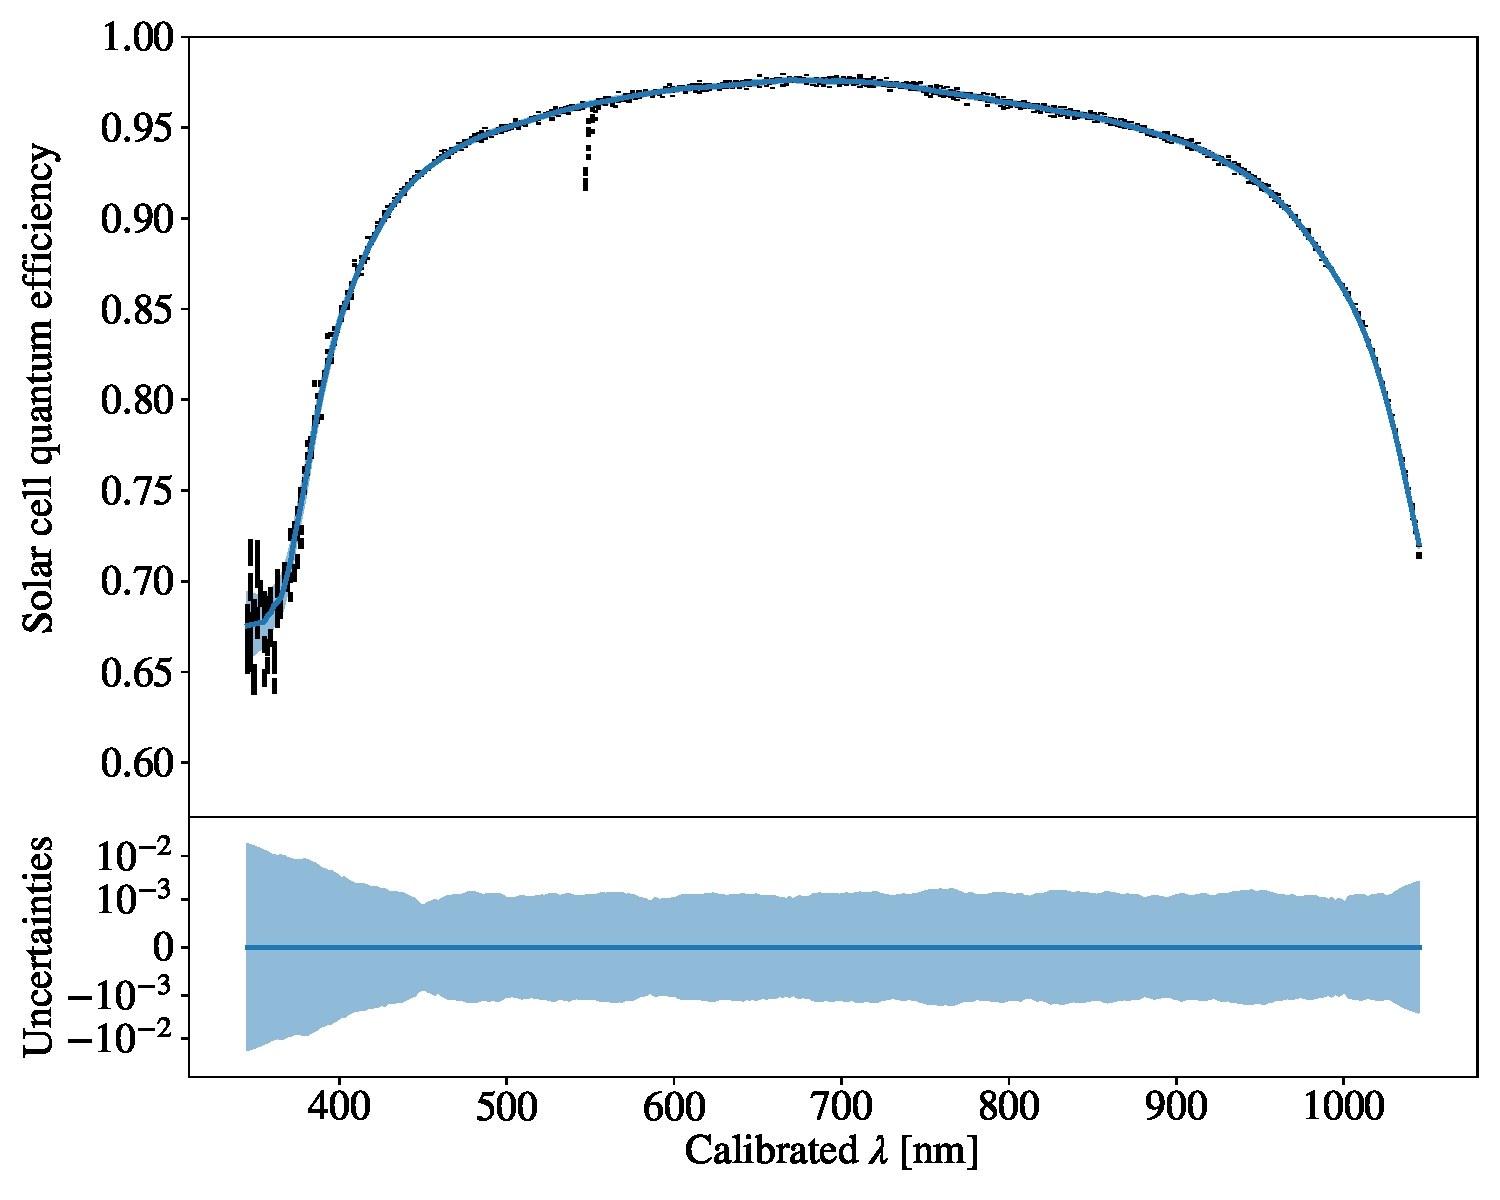
\includegraphics[width=\columnwidth]{solarcell_qe}
\caption{Solar cell quantum efficiency with respect to wavelength (top) and error bar sizes (bottom).}
\end{figure}

\subsubsection{Dark current characterisation}

\todo{Elana : write sentences about the ampere box}

\todo{Jeremy : write a paragraph on the solar cell dark current spectrum}


Connecting the Keysight to a $\SI{243}{\ohm}$ resistor gives exactly the same
correlation function. The dark current comes entirely from the Keysight




%  \begin{figure}[!ht]
%    \begin{center}
%      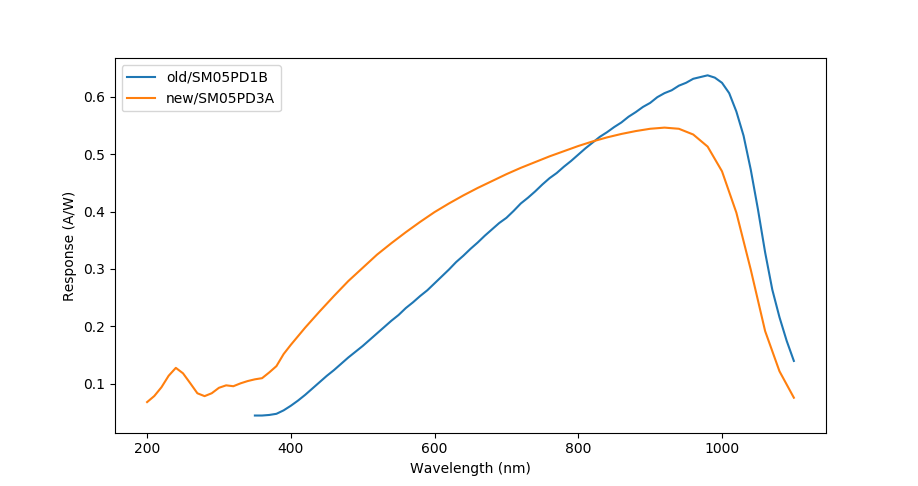
\includegraphics[width=0.8\columnwidth]{thorlabs_response}
%    \end{center}
%    \caption[]{Response curves of the photodiodes. We see the noticeable
%      improvement in the blue for the new one.}
%    \label{fig:thorlabs_response}
%  \end{figure}
%  
%
%
%Sketch and/or images the CBP setting
%
%\begin{itemize}
%\item Ekspla NT252 tunable laser
%\item Light injection system with filters
%\item Optical sphere ref
%\item Ocean QE65000 spectrograph
%\item Photodiode + Keithley 6514. Fig \ref{fig:thorlabs_response}\\
%  \emph{Old one} (used in summer 2021 up to 14th of October 2021): Thorlabs
%  SM05PD1B with FDS100 spectral response data\\
%  \emph{New one} (replaced on the 14th of October 2021): Thorlabs SM05PD3A with
%  FD11A spectral response data
%  
%  
%\item Pinhole slider
%\item Telescope: Ritchey Chretien Omegon telescope\\
%  Apperture ratio $f/9$\\
%  Apperture $154 mm$ \\  
%\item Telescope mount
%\item Solar Cell on movable mount
%\item Keysight B2987A: in order to be able to chop the light at a higher frequency
%  than what the Keithley can do. And it is a more contemporary instrument.
%\end{itemize}

\subsection{Equations and strategy}

\todo{Thierry}

From equations, draw the data taking plan

with calibrated wavelength

\section{CBP response calibration with a solar cell}

\todo{Jérémy}

Foundations: The Solar Cell QE (Sasha and Elana et al.)



\subsection{Preparatory settings}

Before illuminating the solar cell with the CBP, several action has to be taken to maximise the quality of the data sets:
\begin{itemize}
\item place the pinholes at the focus of the CBP telescope
\item tune the telescope iris
\item align the CBP and the solar cell, in position and angle
\item mask every ambient light
\item spectrograph calibration
\item \todo{think a lot about what we forgot}
\end{itemize}



\subsubsection{Focussing}

\todo{Marc}


The CBP was aligned with the StarDICE telescope to improve the focus. The
StarDICE camera was set close to infinity with no filter (focus encoder:
8mm). The smallest pinhole (75microns). Adjustment of the CBP focus was
performed by Elana in order to get the smallest extension of the pinhole
image. A slight offset was then added to account for the small change in focus
introduce by tightening the locking screws. Here is a confirming image taken
just after.

The focus was check to resist slot changes and even complete removing and
reinstallation of the pinhole.

For the record mount coordinates to get CBP and telescope aligned were
$[13.199987411499023, 1.4999985694885254]$


\subsubsection{Iris}

\todo{Marc}


\subsubsection{Alignment of the CBP}

\todo{Thierry}


\subsubsection{Ambient light}

Ambient light can contaminate randomly the sensitive devices depending on their direction in the lab room. We masked all diodes from computers or electronic devices.

\subsubsection{Spectrograph calibration}

\todo{Marc : I would do a test with your software as you fit the 3rd order polynom in one step}

Before and after the main data acquisition run to measure the CBP and \SD responses, we calibrated the spectrograph according to the manufacturer specifications. Light from a Hg-Ar lamp was injected into the integrating sphere to illuminate the spectrograph sensor. The software \texttt{Spectractor} was used to fit the emission lines. The bijection between the fitted centroids and the tabulated line values were fitted by a third order polynomial function as requested by the manufacturer. Only lines with high significance were used XXXXX. In Figure~\ref{fig:} we plot the residuals of the fit, showing a RMS of approximately XXXX resulting in a wavelength calibration uncertainty of .



\begin{figure}[!h]
\centering
%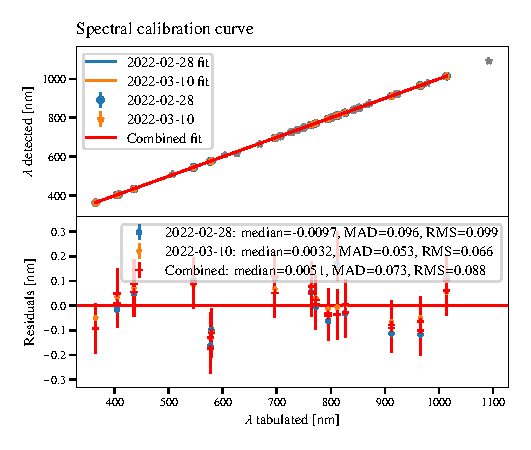
\includegraphics[width=\columnwidth]{spectrograph_calibration}
\caption{Spectrograph calibration plot.}
\end{figure}


During the run, we did not unplug and plug again the optical fibre going from the integrating sphere to the spectrograph. Such an action on the spectrograph side could have changed the wavelength calibration in principle. But beforehand we checked the fibre placement in the spectrograph was very reproducible and do not change the wavelength scale.
 

\subsection{Data set description}


\begin{figure*}[!h]
\centering
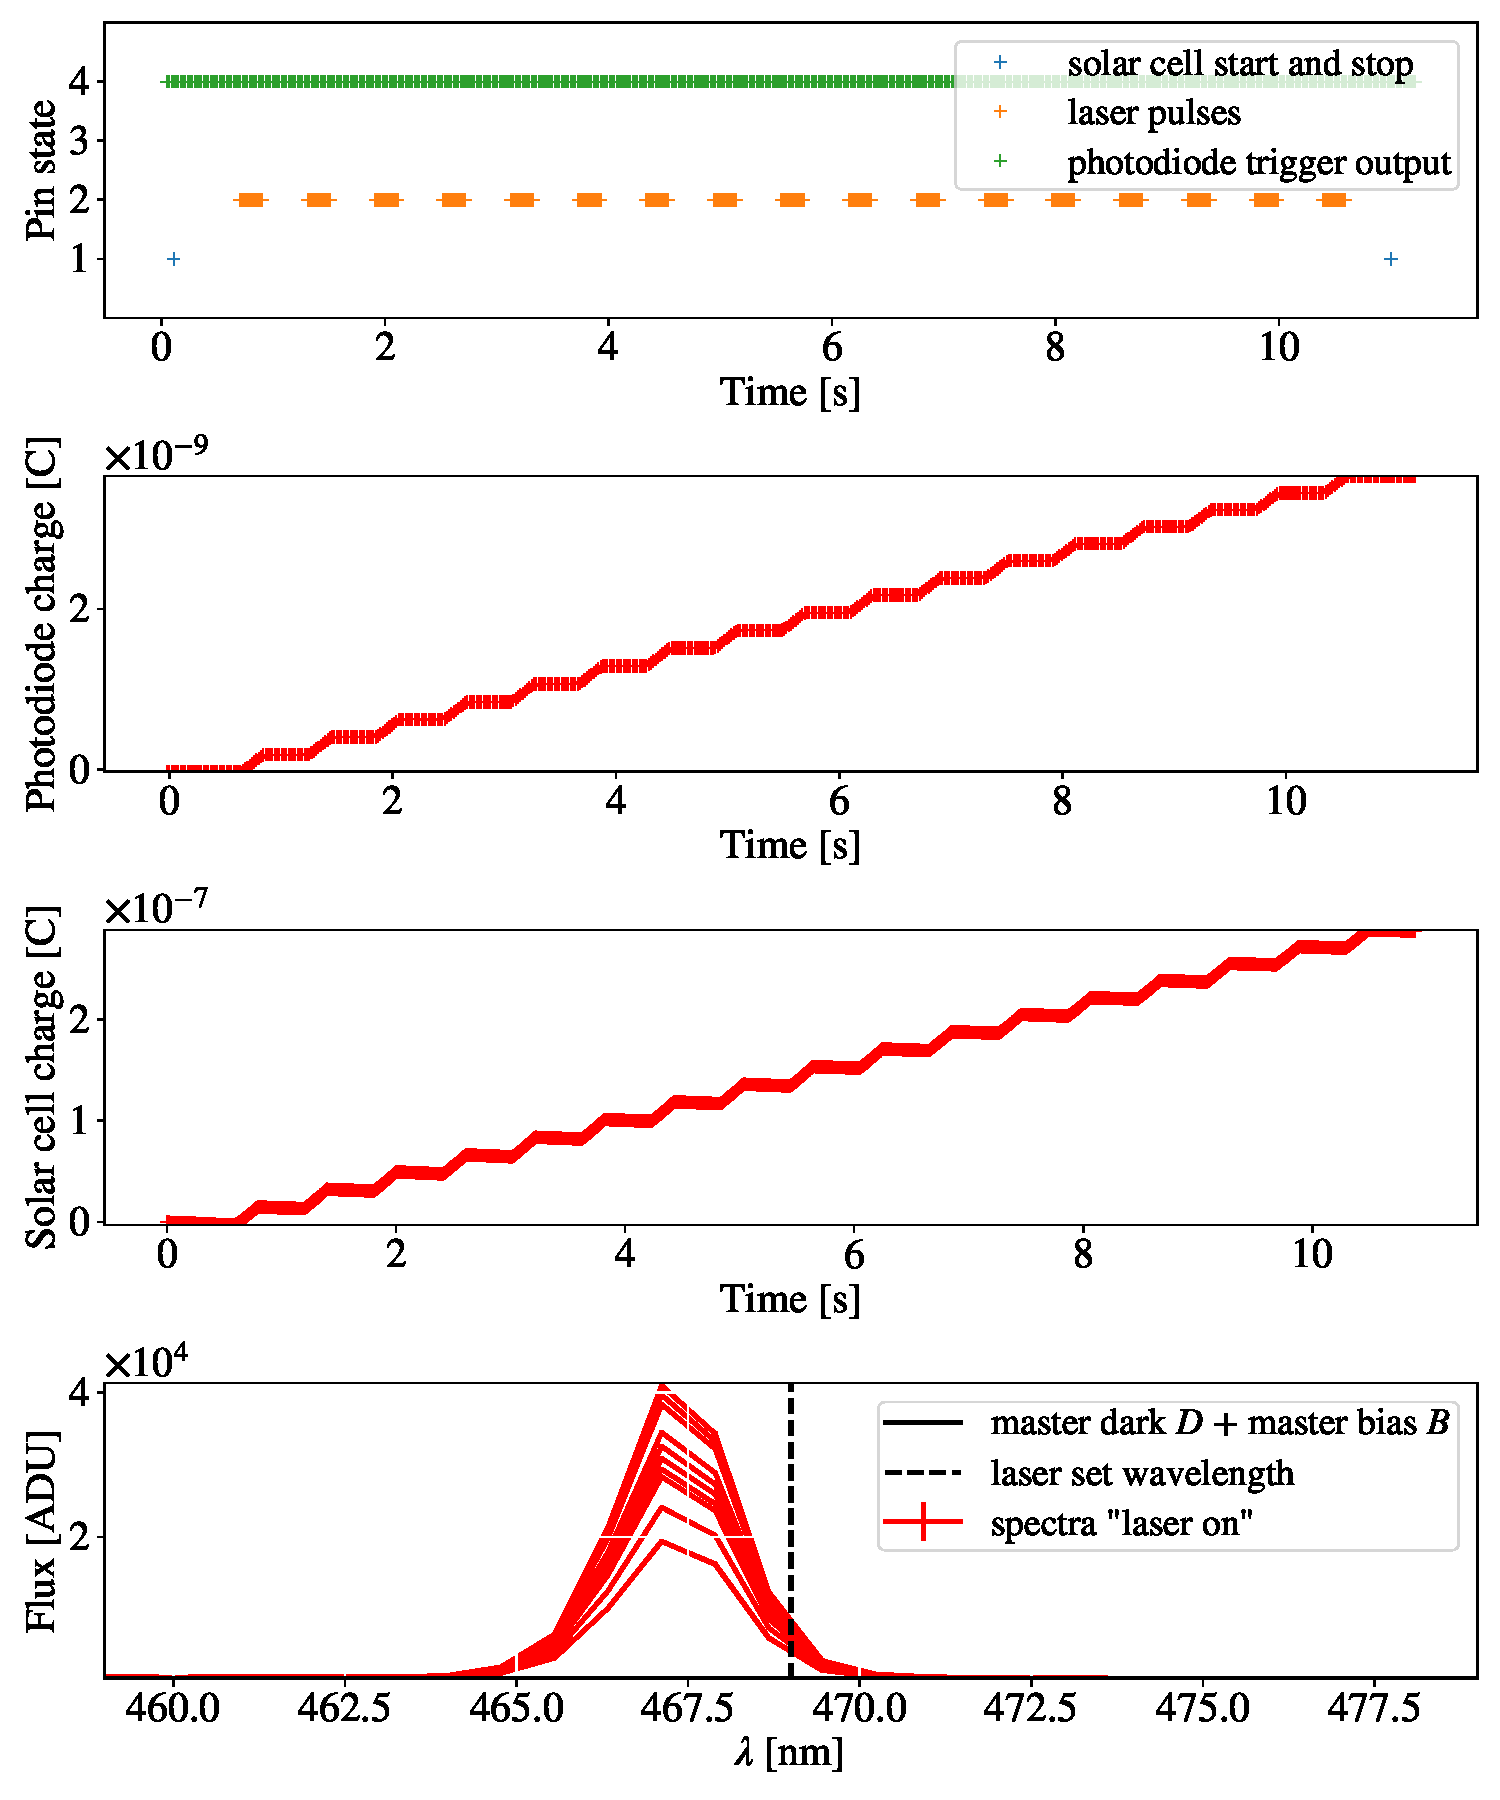
\includegraphics[width=\columnwidth]{sc_dataset_469}
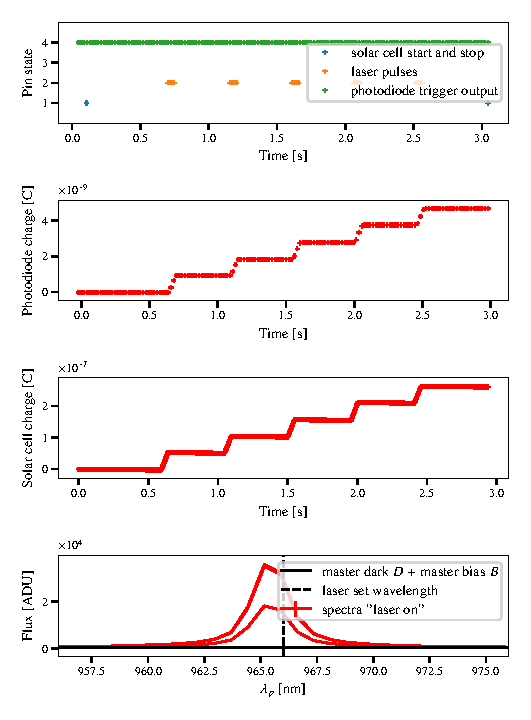
\includegraphics[width=\columnwidth]{sc_dataset_966}
\caption{From top to bottom: typical data sets for digital analyzer (pin state 4 is the Keithley output, pin state 2 the laser trigger output, pin state 1 the Keysight start and end time acquisition time stamps), charges in the photodiode, charges in the solar cell, flux in the spectrograph. Left: typical data set at \SI{469}{\nm}. Right: typical data set at \SI{966}{\nm}.}\label{fig:sc_dataset_examples}
\end{figure*}

The laser emits pulses at a fixed rate of \SI{1}{\kilo\hertz}, with a power that highly depends on the wavelength. To ensure that all instruments work in their linear regime, without saturations, and control the dark current, we decided to shoot light in the solar cell in burst of pulses, separated with dark times at least as long as half the burst length. The number of pulses was set to maintain a rather constant total cumulated charge in the photodiode, which is the common instrument between the CBP and \SD response measurements and the one receiving the maximum power in the system. Therefore we expect to minimize eventual non-linear effects in the instrumental chain. The linearity of the CBP system is checked varying the global laser power in section~\ref{XXX}. However, we know we have a $1/f$ noise in the solar cell instrumental chain. To limit the amplitude of these random fluctuations during the burst, we set the maximum number of pulses to 200, and in that case compensated with higher number of bursts.

A typical dataset to measure the CBP response it the emission of laser bursts in the solar cell, at a given wavelength. Charges in the photodiode and solar cell are recorded jointly, as well as the flux in the spectrograph and the time stamps in the digital analyzer (see examples in Figure~\ref{fig:sc_dataset_examples}).

The charges in the photodiode and the solar cell are read with electrometers in charge mode. This mode is better than the current mode as the integration is performed in a capacitance. This avoids to model the precise current time lines before integrating them numerically, as they are subtlety different from squarewave functions due to different time responses in the system and contaminated by random dark current fluctuations. 

We used the \SI{5}{\mm} pinhole with the largest laser power mode to get the highest signal to noise ratio in the solar cell, but also in the \SD telescope. The solar cell accumulates around \SI{4}{\nano\coulomb} in a burst, with no change of Keysight range, knowing that the dark current fluctuations reaches \SI{6546546}{\nano\coulomb} during a burst duration \todo{a verifier}. The Keysight accuracy in this regime is XXXXXX \todo{to check}. 


During a solar cell measurement run, the laser wavelengths are chosen every nanometre between \SI{350}{\nano\meter} and \SI{1100}{\nano\meter}, but they are randomly shuffled before shooting the laser to avoid that long range $1/f$ modes in the solar cell dark current correlates neighboured data points of the CBP response. Several runs were accumulated to enhance the signal to noise ratio. In particular, five runs were recorded jsut before the \SD telescope measurement, and five new runs were launched just after.


To estimate systematic uncertainties, runs with different settings has been conducted. We varied the laser global power to assess the linearity of the instrumental light and check the ambient light additive contamination. We varied the solar cell distance to estimate the output CBP scattered light.

%\subsubsection{Choice of the dynamic range}
%We need to select the number of pulses per wavelength. We decide to keep the
%photo-diode current as flat as possible in order to keep the non-linearity of
%the Keithley 6514 (that we suppose the largest non-linear component of our
%setup) as small as possible.
%
%
%\begin{figure}[!ht]
%\begin{center}
%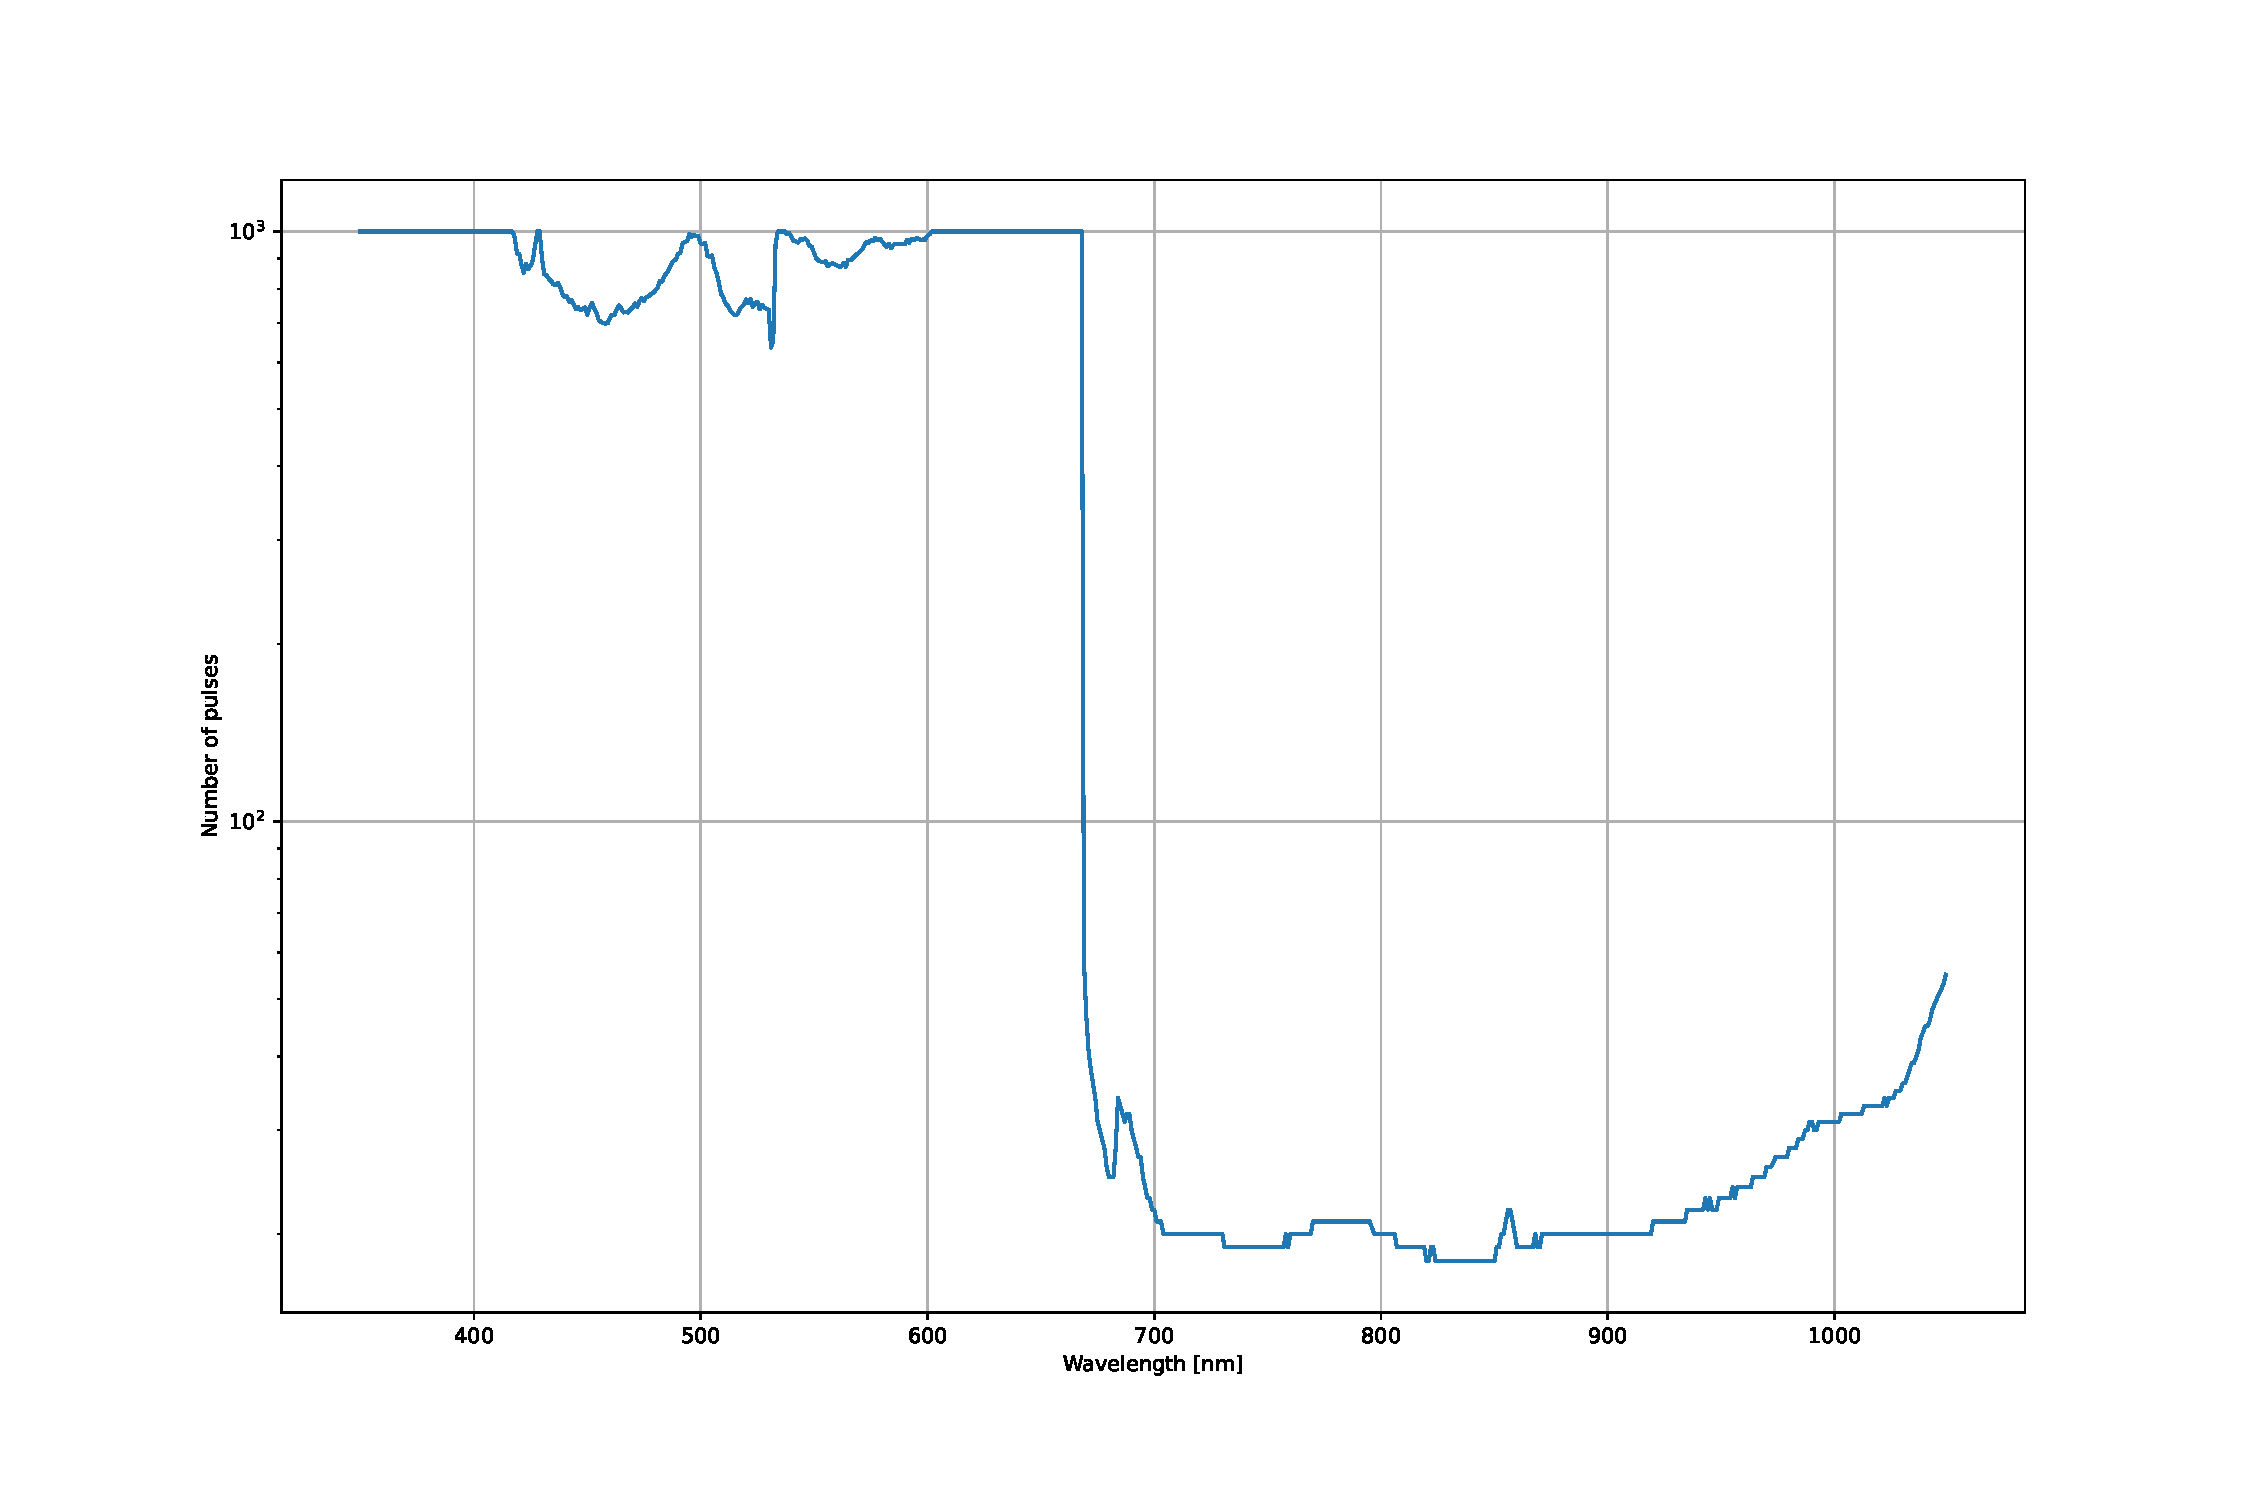
\includegraphics[width=0.8\columnwidth]{calculate_npulses}
%\end{center}
%\caption[]{Number of pulses per bursts needed to get a constant signal from the photodiode.}
%\label{fig:calculate_npulses}
%\end{figure}
%
%This was for the Thorlabs \Oldthorlabs


%\subsubsection{Dark current characterization}
%
%Measurement and selection of a dark current that doesn't saturate the Keisight
%too fast. Measurement of the dark current noise level. 
%
%\begin{itemize}
%\item Without offset box: $\sim 20 nA$
%\item With offset box: $~ <0> nA \pm 5 nA$
%\end{itemize}
%
%
%Dark current with laser off over 45 minutes, mimicking 10 second observation
%blocks corresponding to the 5 laser bursts.
%\begin{figure}[!ht]
%\begin{center}
%%\includegraphics[width=0.8\columnwidth]{dark_current_spectrum.jpeg}
%\end{center}
%\caption[]{Left: signal auto-correlation. Right: signal FFT. Dominated by the
%  stitching of 10 second blocs together.}
%\label{fig:darkcurrentspectrum}
%\end{figure}

%\subsubsection{Current or charge mode}

%\subsubsection{Choice of the pinhole}

%\subsubsection{Masking of the beam}
%We us a $3/4$ pie-slice mask at the end of the CBP telescope in order to reduce
%the beam size, which would otherwile overfill the Solar Cell surface.
%
%Checks to demonstrate that this doesn't impact, via inner reflexions, the
%calibration of the CBP telescope.
%
%
%\subsubsection{Available pinholes}
%
%Choice of a pinhole that allows enough S/N. Since we have to switch pinholes,
%verification of the relation between flux and pinhole size. Verification of
%pinhole achromaticity.
%
%\begin{itemize}
%\item Various pinhole sizes measurements with Solar Cell
%\item Various pinhole sizes measurement with telescope
%\end{itemize}
%


%\subsubsection{Light source filtering}
%
%We suspect that the laser produces harmonics that need to be filtered
%out. Measurement of those harmonics and selection of filters to filter them
%out. 
%



\subsection{Data reduction}

\todo{check that time stamps are explicitly describe in all items}

In a data set, we accumulated several laser bursts. However, a per burst analysis is conducted to be able to remove outliers more easily. All bursts are combined only at the end of the analysis to get the CBP response.

\subsubsection{Photodiode data reduction overview}

We estimated the total charge accumulated in the charge sequence and the leakage currents at beginning and end of the sequence. For the photodiode, the time stamps come directly from the digital analyser clock, with a sampling at XXXXXXXXX \todo{a verifier}. The burst time breaks also. %To estimate the uncertainties on the raw data points are estimated as the RMS around

For each burst, we fit lines during the dark times before and after the burst, removing the closest points to the burst. A $\chi^2$ minimisation is performed using the \texttt{curve\_fit} method from python library \texttt{scipy}. The uncertainties on the data points are adjusted so that the final reduced $\chi^2$ is one. Doing so we assume that the fit residuals are only due to Gaussian instrumental noise, as justified by the Figure~\ref{fig:}. Note that we do not fit anything during the burst time, as the laser power stability do not guaranty that this can be model with a simple mathematical function. We only use the dark times, that we believe they are modelled with straight lines.

We call $t_1$ and $t_2$ the time stamps of the beginning and ending of the laser burst respectively, given by the laser trigger output itself\footnote{Technically, the laser time stamps give the beginning of the pulse, so we add \SI{1}{\ms} to the last trigger time stamps from the laser to account for the pulse duration \todo{mais c'est faux ça ???}}. The accumulated charge $\Delta q_{\rm mes}$ during a burst is then
        $$\Delta q_{\rm mes} = n_2(t_2) - n_1(t_1) - \frac{1}{2} \left[n_1(t_2) - n_1(t_1) + n_2(t_2) - n_2(t_1)  \right]$$
where $n_j(t_i)$ is the line fit of the dark part $j$ (before or after the burst) evaluated at time $t_i$. Doing so, the subtraction $n_2(t_2) - n_1(t_1)$ gives the raw height of the burst step in the charge sequence\footnote{Moreover, doing the subtraction removes systematics inaccuracy coming from the Keithley electrometer.} while the terms in brackets remove the averaged contribution of the dark current using both the dark times before and after the burst. The uncertainties from all line parameters are then propagated to quote the measurement of the charge measured with the photodiode. They are typically of the order of the residual RMS, around \SI{5e-5}{\nano\coulomb}, more than 3 orders of magnitude below the typical $\Delta q_{\rm mes}$ values.



\begin{figure}[!h]
\centering
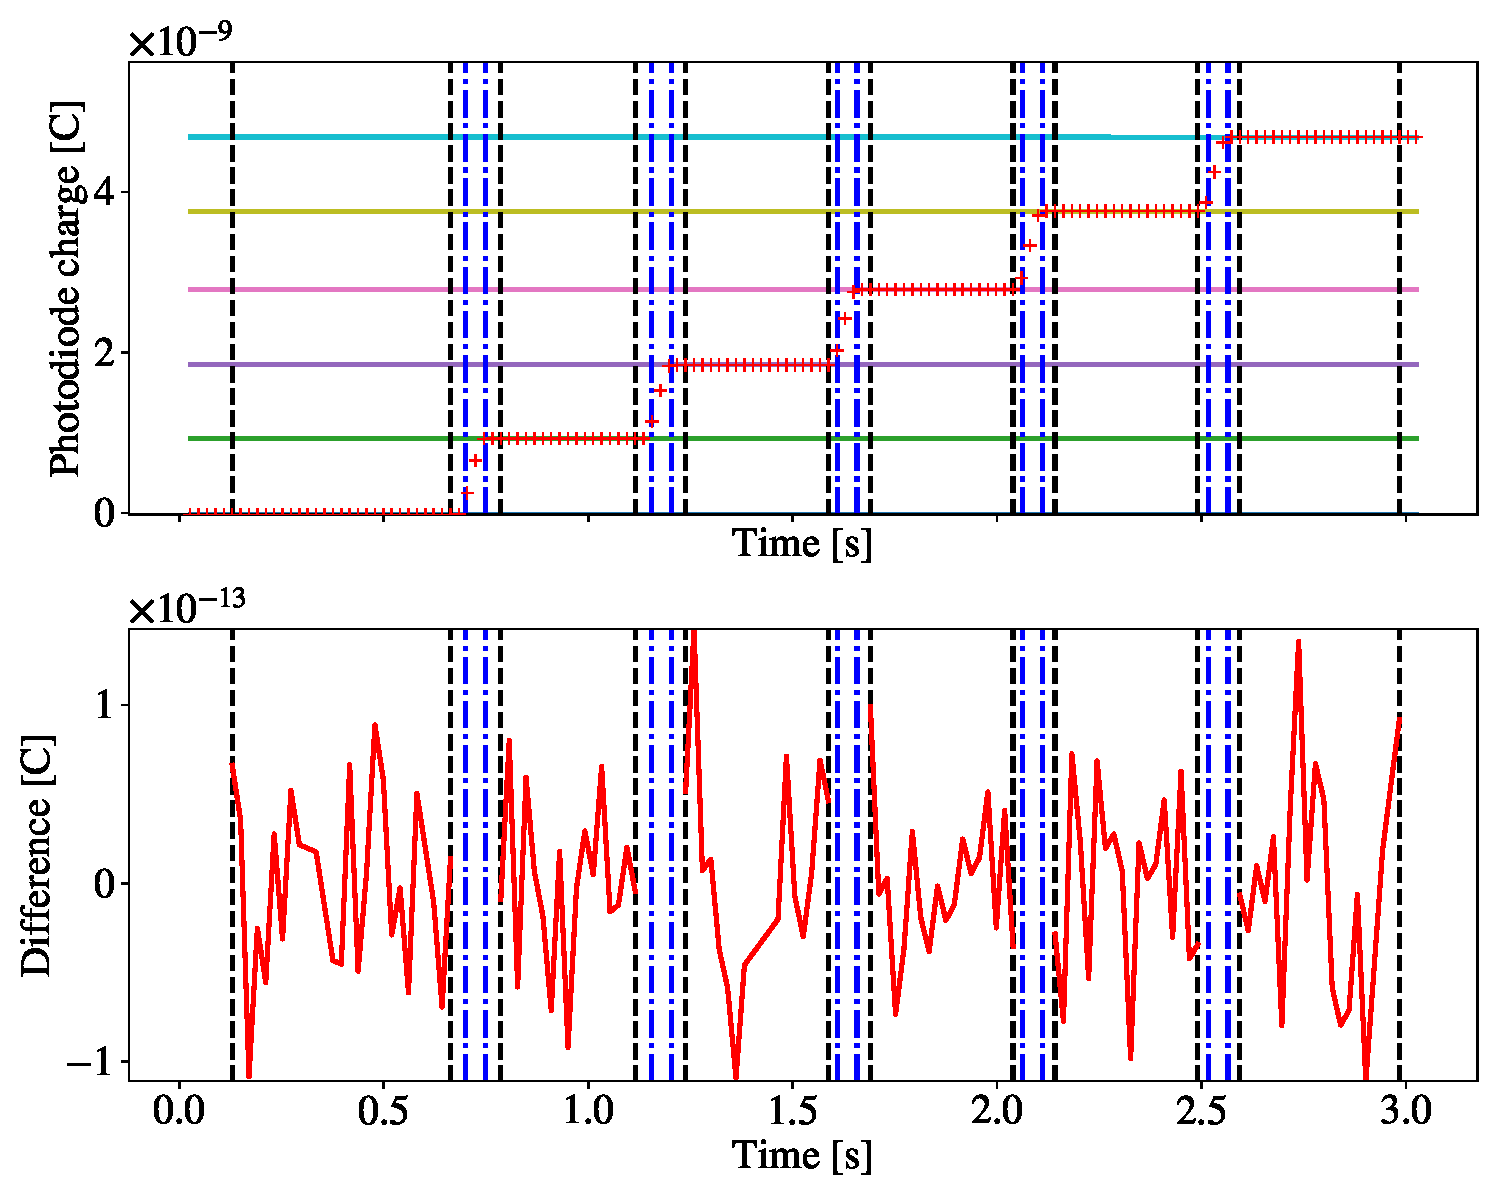
\includegraphics[width=\columnwidth]{pd_reduc_966}
\caption{Photodiode charge sequence reduction process at wavelength \SI{469}{\nm}. Vertical black lines indicates the laser starts and stops, while blue lines flank the dark times. Coloured horizontal lines are fitted during the dark times. The top panel shows the raw charges $q(t)$ acquired with the photodiode, while the bottom panel shows the residuals to the linear fits during the dark times.}
\end{figure}


\subsubsection{Solar cell data reduction overview}

\subsubsection{Spectrograph data reduction overview}

The spectrograph exposure times were set to not reach its saturation level for all wavelengths. However, the sampling rate was not tunable and time stamps unavailable. So we just take as much spectra as we can during an acquisition, and then analyse them. Some contains laser light, other are darks. We assume a spectrum is a dark if they are no spectrograph pixel above its median plus a threshold. To set the threshold, we first compute the RMS per spectrograph wavelength using all the spectra. Then the threshold is the minimum value between either 20\% of the maximum RMS at any wavelength or 20 times the median value of all the RMS values. This setting allows use to detect small and high laser lines, and flag as dark the spectra that do not contain them.

After this repartition of the spectra in two categories, we subtract a bias level and compute a master dark frame doing the median of all the dark spectra. This master dark is subtracted to all spectra. This removes the spectrograph baseline and hot pixels. The spectra containing laser line are them stacked to increase signal to noise ratio of the line and of the contaminations.

Then we use the \texttt{Spectractor} software to detect emission lines and fit their centroids. We searched for the laser line of course, but also lines at \SI{532}{\nm} and from two photon conversions. Indeed, we noticed the presence of a \SI{532}{\nm} line in the regime 532 to \SI{669}{\nm}, and of a weak line when the laser is set to wavelength above \SI{1064}{\nm}. If we call $\lambda_L$ the laser wavelength, we observed the production of photons at wavelength $\lambda_h$ given by
\begin{equation}
 \frac{2}{\SI{1064}{\nm}} = \frac{1}{\lambda_L} + \frac{1}{\lambda_h}
 \end{equation} 
due to the conversion of two \SI{1064}{\nm} photons into a laser photon at $\lambda_L$ and a complementary photon at $\lambda_h$ that ended in the laser beam. In practice, we observed a small emission line in the spectrograph when $\lambda_L > \SI{1064}{\nm}$, nearly symmetrical of the laser line with respect to \SI{1064}{\nm}. An example of a stacked spectra with the detection of the laser line at \SI{643}{\nm} and the pump line at \SI{532}{\nm} is shown in Figure~\ref{fig:spectro_reduc_643}.




\begin{figure}[!h]
\centering
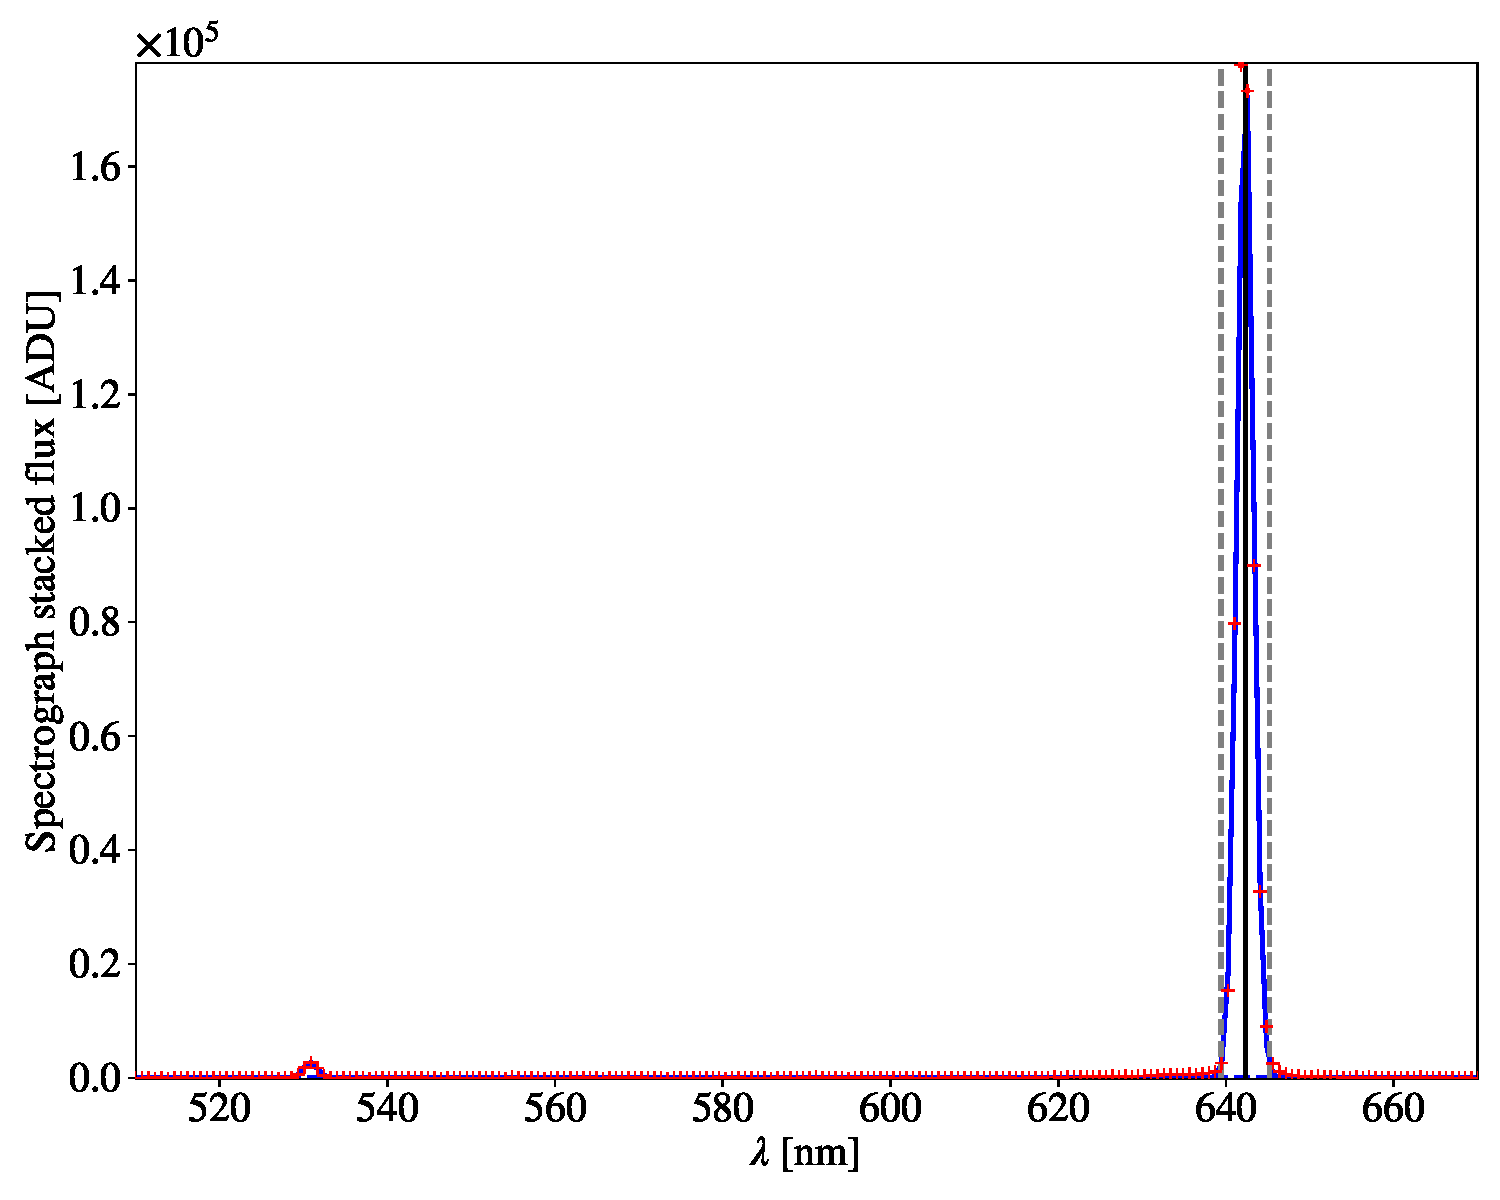
\includegraphics[width=\columnwidth]{spectro_reduc_643}
\caption{Fit of Gaussian profiles in the stacked spectra for a laser line at $\lambda_L=\SI{643}{\nm}$. The contamination line at \SI{532}{nm} is also visible.}\label{fig:spectro_reduc_643}
\end{figure}


Using \texttt{Spectractor} and the spectrograph calibration, we then have the true laser wavelength at the Angstrom level. Indeed the realised wavelength is never the one a priori asked, as one can see in Figure~\ref{fig:sc_dataset_examples}. However, we observed a remarkable repeatability of the correspondence between the set wavelength and the realised wavelength (see Figure~\ref{fig:wavelength_stability}). Therefore, in most figures of this paper we use the set laser wavelength. 

\todo{Jérémy : to improve : recovery of lines close to the sensor edges, check the stabitilty with time after spline subtraction and interpolation in regions contaminated by lines}




\begin{figure}[!h]
\centering
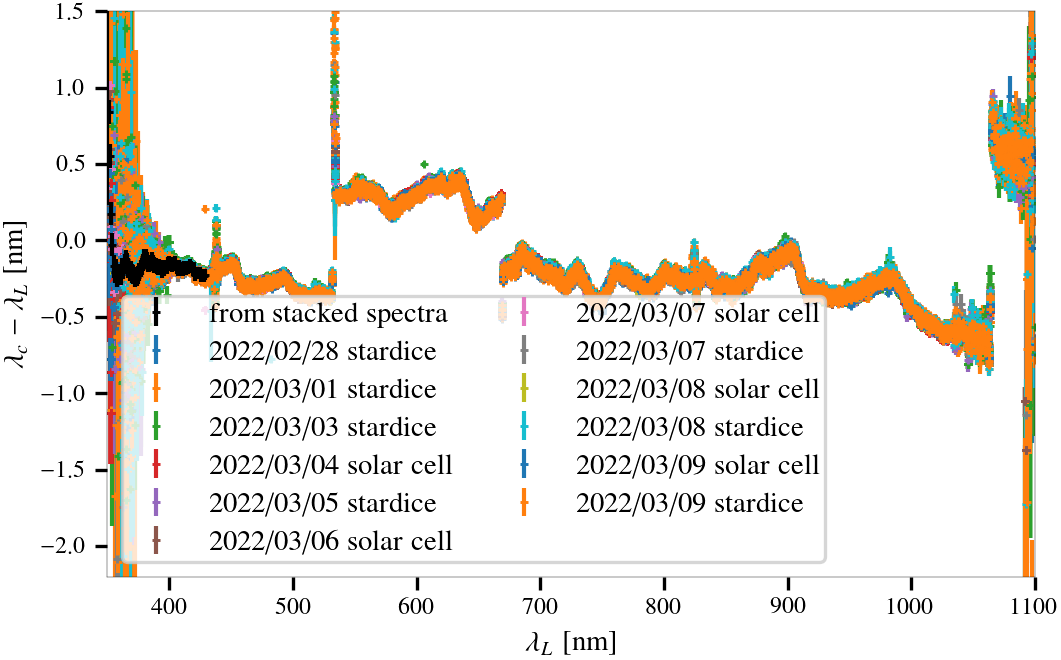
\includegraphics[width=\columnwidth]{wavelength_stability}
\caption{Difference between the detected and requested laser wavelengths, for all the $\approx 86000$ data sequences acquired in our acquisition run.}\label{fig:wavelength_stability}
\end{figure}

\subsection{CBP response}

\subsection{Systematics}

\subsubsection{Wavelength calibration}

\todo{Jérémy : misknowledge of wavelengths close to sensor edges, 532 and 1064}


\subsubsection{Laser light contamination}

\todo{Jeremy : light from 532 or 1064 to remove from photodiode and solar cell, indirect light from laser burst}

\subsubsection{Ambient light and instrumental chain linearity check}

\todo{Jeremy : QSW ratios}

Varying QSW we assume that seen non-linearities come from an external light component

The Solar Cell has small shunt resistance and we light it with a powerful source
of very short pulse length. Verification of linearity w.r.t flux and w.r.t
number of pulses per burst. 


\begin{itemize}
  \item QSW sequence  (Fig. \ref{fig:SCqswlinearity})
  \item Behavior with change of number of pulses
  \item Behavior of solar cell at different distances
\end{itemize}


\begin{figure}[!ht]
\begin{center}
\includegraphics[width=0.8\columnwidth]{solar_cell_qsw_linearity.jpg}
\end{center}
\caption[]{Something}
\label{fig:SCqswlinearity}
\end{figure}


\subsubsection{CBP scattered light varying the solar cell distance}


\subsubsection{Solar cell QE variations with angle and temperature}

\todo{Do we write here the results ?}


\subsubsection{Summary}


\section{Instrument model}\label{sec:model}

\todo{Marc: mais plus tard après analyse, et/ou après tuto}

\todo{Direct transmission measurement, ghost brightness model, angle dependence,  Pupil synthesis}

\section{Stardice response}
\label{sec:dataset}

\subsection{Data set description}
\label{sec:datadesc}

\begin{itemize}
\item Images
\item Photocurrent timeseries
\item Spectral time series
\end{itemize}

\subsection{Reduction of images}
\label{sec:photometry}

\todo{phrase pour dire que c'est pareil pour photodiode et spectro}

\subsubsection{5mm pinhole}

\subsubsection{75um pinhole}

\subsubsection{Ghost photometry}

\subsection{Stardice sky response}

\subsubsection{CCD grid}

\subsubsection{Mirror scan}

\subsubsection{Radius scan}

\subsubsection{Ghost buster and beam impact}

\subsubsection{On sky pupil synthesis and filters}



\subsection{Systematic uncertainties}
\label{sec:systematics}

\subsubsection{Stability of the StarDice responses}

\subsubsection{Gain and linearity}
\label{sec:gain}

Varying pinhole with StarDice, and CBP

Varying QSW but depending on result it falls into this subsection or the following

\subsubsection{Pinhole chromaticity}

\subsubsection{Pull distributions}

\subsubsection{Courbes de croissances}


\section{Discussion}

\section{Conclusion}
\label{sec:conclusion}



\begin{acknowledgements}
We are grateful to ...
\end{acknowledgements}


\bibliographystyle{aa}
\bibliography{cbp}

\appendix

\end{document}

